\documentclass[../main.tex]{subfiles}
\begin{document}
%=========================================================
% TĐ_PBT_PRE1_HK1_Tuan16
% Phiếu bài tập PRE1 - Tuần 16
%   Toán: Phép trừ trong phạm vi 5 (tiếp theo)
%   Tiếng Việt: Làm quen âm c, x
% Soạn theo mẫu (\hktuan, bt)
% Hình màu đặt trong thư mục Hinh_PRE1_Tuan16/ (cùng cấp với file này), tên hình có tiền tố p16_
% Đường dẫn tính từ thư mục của main.tex khi biên dịch main.tex
\graphicspath{{Hinh_PRE1_Tuan16/}{Data_PhieuBaiTap_HK0/Hinh_PRE1_Tuan16/}}
%=========================================================

%---------- Lệnh dùng chung cho phiếu ----------
% Chỗ chấm điền
\providecommand{\TTcham}[1][3cm]{\makebox[#1]{\dotfill}}
% Dòng thông tin học sinh
\providecommand{\TTthongtin}{%
  \noindent\begin{tabular}{|p{7.6cm}|p{4cm}|p{4cm}|}
    \hline
    \textbf{Họ và tên HS:}\dotfill & \textbf{Lớp:}\dotfill & \textbf{Ngày:}\dotfill \\
    \hline
  \end{tabular}\par\medskip}
% Đánh lại số bài từ 1 cho phiếu Tiếng Việt (chỉ khi môi trường bt có bộ đếm tên bt)
\makeatletter
\providecommand{\TTdatlaibai}{\@ifundefined{c@bt}{}{\setcounter{bt}{0}}}
\makeatother
% Bắt đầu phần hình vẽ ngay dưới đề bài (không tách trang giữa đề và hình)
\providecommand{\TTbatdauhinh}{}\renewcommand{\TTbatdauhinh}{\par\nopagebreak\vspace{4pt}\nopagebreak}
% Khoảng cách giữa hai bài
\providecommand{\TTcachbai}{}\renewcommand{\TTcachbai}{\vspace{6pt}}

%---------- Màu dùng cho hình vẽ ----------
\definecolor{PKdo}{RGB}{230,60,60}\definecolor{PKxanhla}{RGB}{90,180,80}
\definecolor{PKxanhdam}{RGB}{20,90,190}\definecolor{PKvang}{RGB}{255,205,60}
\definecolor{PKvangnhat}{RGB}{255,243,190}\definecolor{PKcam}{RGB}{255,150,60}
\definecolor{PKhong}{RGB}{255,140,180}\definecolor{PKnau}{RGB}{140,85,45}
\definecolor{PKxanhnuoc}{RGB}{90,170,235}
\definecolor{PQkem}{RGB}{255,250,235}\definecolor{PQcat}{RGB}{238,214,160}
\definecolor{PQtim}{RGB}{150,90,200}\definecolor{PQngoc}{RGB}{20,170,170}
\definecolor{PQthong}{RGB}{40,140,70}\definecolor{PQda}{RGB}{255,214,180}
\definecolor{PQmauli}{RGB}{70,150,170}\definecolor{PQmaulidam}{RGB}{35,85,100}

%%%%%%%%%%%%%%%%%%%%%%%%%%%%%%%%%%%%%%%%%%%%%%%%%%%%%%%%%%
%   HÌNH VẼ TIKZ (mỗi hình vẽ tại gốc tọa độ, đặt bằng scope shift)
%%%%%%%%%%%%%%%%%%%%%%%%%%%%%%%%%%%%%%%%%%%%%%%%%%%%%%%%%%
% Dấu trừ và dấu bằng nét tròn đầu: \PQtru, \PQbang (vẽ tại gốc)
\providecommand{\PQtru}{}\renewcommand{\PQtru}{\draw[line width=3.2pt,line cap=round] (-0.24,0)--(0.24,0);}
\providecommand{\PQbang}{}\renewcommand{\PQbang}{\draw[line width=3.2pt,line cap=round] (-0.24,0.13)--(0.24,0.13) (-0.24,-0.13)--(0.24,-0.13);}
% Ô trống để điền: \PQo{x,y}{nội dung}
\providecommand{\PQo}{}\renewcommand{\PQo}[2]{\node[draw,line width=1.3pt,rounded corners=5pt,minimum size=1.05cm,fill=white,font=\sffamily\LARGE] at (#1) {#2};}

% ---- Bài bàn tay: \PQphepTay{hình tay 1}{hình tay 2}
\providecommand{\PQphepTay}{}\renewcommand{\PQphepTay}[2]{%
  \begin{tikzpicture}
    \fill[PKvangnhat!55,draw=PKcam!70,thick,rounded corners=10pt] (-0.72,-1.1) rectangle (4.78,1.1);
    \node[inner sep=0pt] at (0,0) {\includegraphics[height=1.8cm]{#1}};
    \begin{scope}[shift={(1.0,0)},scale=0.8]\PQtru\end{scope}
    \node[inner sep=0pt] at (2.0,0) {\includegraphics[height=1.8cm]{#2}};
    \begin{scope}[shift={(3.0,0)},scale=0.8]\PQbang\end{scope}
    \node[draw,line width=1.5pt,rounded corners=8pt,minimum size=1.15cm,fill=white] at (4.02,0) {};
  \end{tikzpicture}}

% ---- Cá trắng (nét viền, để bé tô màu), đầu quay sang phải, dài khoảng 1,35
\providecommand{\PQcatrang}{}\renewcommand{\PQcatrang}{%
  \begin{scope}[line join=round,draw=black!80,thick]
  \filldraw[fill=white] (-0.38,0) .. controls (-0.5,0.12) .. (-0.76,0.34) .. controls (-0.66,0.14) and (-0.56,0.05) .. (-0.53,0)
     .. controls (-0.56,-0.05) and (-0.66,-0.14) .. (-0.76,-0.34) .. controls (-0.5,-0.12) .. (-0.38,0) -- cycle;
  \draw[thin] (-0.44,0.03)--(-0.64,0.2) (-0.44,-0.03)--(-0.64,-0.2);
  \filldraw[fill=white] (-0.3,0.15) .. controls (-0.22,0.36) and (0.02,0.38) .. (0.2,0.24) -- cycle;
  \filldraw[fill=white] (-0.08,-0.2) .. controls (-0.05,-0.34) and (0.06,-0.34) .. (0.1,-0.21) -- cycle;
  \filldraw[fill=white] (0.58,0) .. controls (0.5,0.3) and (-0.1,0.34) .. (-0.4,0.06) -- (-0.4,-0.06) .. controls (-0.1,-0.32) and (0.5,-0.28) .. (0.58,0);
  \draw (0.3,0.19) .. controls (0.24,0.08) and (0.24,-0.08) .. (0.3,-0.18);
  \filldraw[fill=white,thin] (0.42,0.07) circle (0.065);
  \fill[black] (0.435,0.07) circle (0.035);
  \draw[line cap=round] (0.58,0) -- (0.52,-0.03);
  \end{scope}}

% ---- Bể cá tròn có cá trắng: \PQbinhca{danh sách x/y/hướng (1 hoặc -1)}{số bị trừ}{số trừ}
\providecommand{\PQbinhca}{}\renewcommand{\PQbinhca}[3]{%
  \begin{tikzpicture}[line join=round]
    \def\PQthanbinh{(-0.8,1.62) .. controls (-0.62,1.5) .. (-0.68,1.28) arc[start angle=118,end angle=422,radius=1.45] .. controls (0.62,1.5) .. (0.8,1.62)}
    \fill[gray!22] (0,-1.47) ellipse (1.15 and 0.13);
    \begin{scope}
      \clip \PQthanbinh -- cycle;
      \fill[white] (-1.6,-1.6) rectangle (1.6,1.7);
      \fill[top color=PKxanhnuoc!10,bottom color=PKxanhnuoc!35] (-1.6,-1.5) -- (-1.6,0.98) .. controls (-0.6,1.06) and (0.4,0.9) .. (1.6,1.0) -- (1.6,-1.5) -- cycle;
      \fill[PQcat] (-1.6,-1.6) -- (-1.6,-0.93) .. controls (-0.5,-0.78) and (0.5,-1.08) .. (1.6,-0.9) -- (1.6,-1.6) -- cycle;
      \foreach \x/\y/\m in {-0.85/-1.08/gray!45,-0.55/-1.2/PKcam!40,-0.1/-1.12/gray!35,0.35/-1.22/PKxanhnuoc!45,0.75/-1.05/gray!50,0.1/-1.32/PKhong!45}{
        \fill[\m] (\x,\y) ellipse (0.11 and 0.07);}
      \fill[PQthong!75] (0.92,-0.95) .. controls (0.75,-0.6) and (1.05,-0.35) .. (0.88,0.02) .. controls (1.12,-0.35) and (0.9,-0.6) .. (1.02,-0.95) -- cycle;
      \fill[PQthong!60] (1.02,-0.95) .. controls (1.2,-0.7) and (1.05,-0.5) .. (1.2,-0.3) .. controls (1.25,-0.55) and (1.15,-0.75) .. (1.1,-0.95) -- cycle;
    \end{scope}
    \draw[PKxanhnuoc!80!black,thin] (-1.05,1.0) .. controls (-0.6,1.06) and (0.4,0.9) .. (1.04,1.0);
    \draw[PKxanhdam!70!black,line width=1.3pt] \PQthanbinh;
    \filldraw[fill=PKxanhnuoc!10,draw=PKxanhdam!70!black,line width=1.3pt] (0,1.62) ellipse (0.8 and 0.1);
    \draw[white,line width=3.2pt,line cap=round,opacity=0.9] (150:1.2) arc (150:200:1.2);
    \draw[white,line width=2pt,line cap=round,opacity=0.9] (207:1.2) arc (207:214:1.2);
    \foreach \x/\y/\h in {#1}{\begin{scope}[shift={(\x,\y)},xscale=0.6*\h,yscale=0.6]\PQcatrang\end{scope}}
    \foreach \x/\y/\r in {0.55/0.82/0.045,0.62/0.68/0.03,-0.75/0.85/0.035}{\draw[PKxanhnuoc!80!black,thin,fill=white] (\x,\y) circle (\r);}
    \node[font=\sffamily\LARGE,anchor=east] at (0.55,-2.05) {#2 $-$ #3 $=$};
    \PQo{1.25,-2.05}{}
  \end{tikzpicture}}

% ---- Cần câu có ghi phép tính: \PQcancau{phép tính}
\providecommand{\PQcancau}{}\renewcommand{\PQcancau}[1]{%
  \begin{tikzpicture}[line cap=round,line join=round]
    \draw[PKcam!85!black,line width=2.2pt] (0.12,0.35) .. controls (0.45,1.45) and (1.35,2.05) .. (2.55,2.1);
    \foreach \t/\x/\y in {1/0.55/1.18,2/1.2/1.78,3/1.9/2.06}{\draw[gray!60!black,thin] (\x,\y) circle (0.045);}
    \draw[black!85,thick] (0.62,0.58) .. controls (0.6,0.9) and (0.45,1.0) .. (0.55,1.13)
      .. controls (0.8,1.15) and (0.95,1.35) .. (1.2,1.73) .. controls (1.45,1.75) and (1.6,1.95) .. (1.9,2.01)
      .. controls (2.2,1.98) and (2.35,2.05) .. (2.55,2.1)
      .. controls (2.7,1.7) and (2.45,1.25) .. (2.62,0.8);
    \draw[PKcam!85!black,very thick] (2.62,0.8) -- (2.62,0.6) arc (0:-200:0.11);
    \draw[PKcam!85!black,thin,fill=white] (2.62,0.84) circle (0.045);
    \draw[PKcam!55!black,line width=7pt] (-0.06,-0.3) -- (0.14,0.38);
    \draw[PKcam!35!black,thin] (-0.02,-0.12)--(0.08,-0.15) (0.02,0.02)--(0.12,-0.01) (0.06,0.16)--(0.16,0.13);
    \shade[ball color=black!75] (0.62,0.36) circle (0.25);
    \foreach \g in {45,135,225,315}{\fill[white] ($(0.62,0.36)+(\g:0.12)$) circle (0.035);}
    \draw[black!80,thick] (0.4,0.42) -- (0.22,0.38);
    \node[draw,densely dashed,thick,rounded corners=6pt,minimum width=2.7cm,minimum height=1.0cm,fill=white,font=\sffamily\bfseries\LARGE] at (1.25,-0.75) {#1};
    \fill (1.25,-1.45) circle (2.6pt);
  \end{tikzpicture}}

% ---- Cá vàng có ghi số trong vòng tròn: \PQcaso{số}
\providecommand{\PQcaso}{}\renewcommand{\PQcaso}[1]{%
  \begin{tikzpicture}[line join=round,scale=1.75]
    \fill[PKcam,draw=PKcam!55!black,thick] (-0.38,0) .. controls (-0.5,0.12) .. (-0.76,0.34) .. controls (-0.66,0.14) and (-0.56,0.05) .. (-0.53,0)
       .. controls (-0.56,-0.05) and (-0.66,-0.14) .. (-0.76,-0.34) .. controls (-0.5,-0.12) .. (-0.38,0) -- cycle;
    \draw[PKcam!45!black,thin] (-0.44,0.02)--(-0.66,0.2) (-0.44,-0.02)--(-0.66,-0.2) (-0.45,0)--(-0.6,0);
    \fill[PKcam,draw=PKcam!55!black,thick] (-0.3,0.15) .. controls (-0.22,0.38) and (0.02,0.4) .. (0.22,0.24) -- cycle;
    \fill[PKcam,draw=PKcam!55!black,thick] (-0.08,-0.2) .. controls (-0.05,-0.34) and (0.06,-0.34) .. (0.1,-0.21) -- cycle;
    \path[top color=PKvang!90!orange,bottom color=PKvang!45!white,draw=PKcam!55!black,thick]
       (0.58,0) .. controls (0.5,0.3) and (-0.1,0.34) .. (-0.4,0.06) -- (-0.4,-0.06) .. controls (-0.1,-0.32) and (0.5,-0.28) .. (0.58,0);
    \fill[white,opacity=0.5] (0.05,0.17) ellipse (0.16 and 0.04);
    \fill[white,draw=black!70,densely dashed,thin] (-0.02,-0.01) circle (0.2);
    \node[font=\sffamily\bfseries\large] at (-0.02,-0.01) {#1};
    \fill[white,draw=PKcam!45!black,thin] (0.4,0.06) circle (0.07);
    \fill[black] (0.415,0.06) circle (0.04);
    \fill[white] (0.428,0.078) circle (0.013);
    \draw[PKcam!45!black,thick,line cap=round] (0.56,-0.05) .. controls (0.52,-0.1) .. (0.47,-0.09);
    \fill[PKcam!90!black,opacity=0.9] (0.24,-0.06) .. controls (0.1,-0.02) and (0.08,-0.14) .. (0.12,-0.17) .. controls (0.18,-0.14) .. (0.24,-0.06);
    \fill (-0.02,0.5) circle (1.5pt);
  \end{tikzpicture}}

% ---- Quả táo dễ thương có mặt cười (vẽ tại gốc, rộng khoảng 1,25)
\providecommand{\PQtaoxinh}{}\renewcommand{\PQtaoxinh}{%
  \def\PQvotao{(0,0.4) .. controls (-0.2,0.55) and (-0.62,0.5) .. (-0.62,0.05) .. controls (-0.62,-0.4) and (-0.3,-0.58) .. (-0.12,-0.5) .. controls (-0.05,-0.47) and (0.05,-0.47) .. (0.12,-0.5) .. controls (0.3,-0.58) and (0.62,-0.4) .. (0.62,0.05) .. controls (0.62,0.5) and (0.2,0.55) .. (0,0.4)}
  \shade[inner color=red!55,outer color=red!85!black] \PQvotao;
  \draw[red!45!black,thin] \PQvotao;
  \fill[white,opacity=0.55] (-0.36,0.2) ellipse (0.07 and 0.13);
  \draw[PKnau!80!black,line width=1.6pt,line cap=round] (0,0.4) .. controls (0.02,0.52) .. (0.07,0.62);
  \shade[top color=green!65!black,bottom color=green!45!yellow,rotate around={28:(0.24,0.6)}] (0.24,0.6) ellipse (0.2 and 0.08);
  \draw[green!35!black,thin,rotate around={28:(0.24,0.6)}] (0.06,0.6) -- (0.4,0.6);
  \fill[black] (-0.2,0.0) ellipse (0.055 and 0.075); \fill[black] (0.2,0.0) ellipse (0.055 and 0.075);
  \fill[white] (-0.18,0.03) circle (0.02); \fill[white] (0.22,0.03) circle (0.02);
  \fill[PKhong!80,opacity=0.75] (-0.34,-0.13) ellipse (0.08 and 0.045); \fill[PKhong!80,opacity=0.75] (0.34,-0.13) ellipse (0.08 and 0.045);
  \draw[black,thick,line cap=round] (-0.08,-0.12) .. controls (-0.04,-0.19) and (0.04,-0.19) .. (0.08,-0.12);}

% ---- Đầu thỏ ló lên sau mép khung (vẽ tại gốc): \PQthoLo{nghiêng}
\providecommand{\PQthoLo}{}\renewcommand{\PQthoLo}[1]{%
  \begin{scope}[rotate=#1,line join=round]
    \filldraw[fill=PQkem,draw=black!70,thick,rotate around={14:(-0.24,0.78)}] (-0.24,0.78) ellipse (0.15 and 0.42);
    \fill[PKhong!70,rotate around={14:(-0.24,0.8)}] (-0.24,0.8) ellipse (0.07 and 0.3);
    \filldraw[fill=PQkem,draw=black!70,thick,rotate around={-14:(0.24,0.78)}] (0.24,0.78) ellipse (0.15 and 0.42);
    \fill[PKhong!70,rotate around={-14:(0.24,0.8)}] (0.24,0.8) ellipse (0.07 and 0.3);
    \filldraw[fill=PQkem,draw=black!70,thick] (0,0.12) ellipse (0.5 and 0.4);
    \fill[black] (-0.17,0.18) circle (0.05); \fill[black] (0.17,0.18) circle (0.05);
    \fill[white] (-0.155,0.2) circle (0.016); \fill[white] (0.185,0.2) circle (0.016);
    \fill[PKhong!90!red] (0,0.08) ellipse (0.05 and 0.035);
    \draw[black!80,thin] (0,0.05) -- (0,0.0) (-0.08,-0.03) .. controls (-0.04,-0.06) .. (0,0.0) .. controls (0.04,-0.06) .. (0.08,-0.03);
    \fill[PKhong!60,opacity=0.8] (-0.3,0.03) ellipse (0.08 and 0.045); \fill[PKhong!60,opacity=0.8] (0.3,0.03) ellipse (0.08 and 0.045);
  \end{scope}}
\providecommand{\PQchanTho}{}\renewcommand{\PQchanTho}{% bàn chân thỏ bám mép khung
  \filldraw[fill=PQkem,draw=black!70,thick] (-0.12,0) arc (180:0:0.12) -- cycle;
  \draw[black!60,thin] (-0.04,0) -- (-0.04,0.06) (0.04,0) -- (0.04,0.06);}

% ---- Một hàng gạch táo: \PQhangtao{số táo}{số bị trừ}{số trừ}
\providecommand{\PQhangtao}{}\renewcommand{\PQhangtao}[3]{%
  \draw[line width=1.3pt,rounded corners=6pt,fill=white] (0,-0.9) rectangle (13.6,0.9);
  \foreach \k in {1,...,#1}{\begin{scope}[shift={({3.35+(\k-(#1+1)/2)*1.15},-0.05)},scale=0.8]\PQtaoxinh\end{scope}}
  \node[font=\sffamily\bfseries\LARGE,anchor=east] at (10.5,0) {#2 $-$ #3 $=$};
  \PQo{11.6,0}{}}

% ---- Cây táo trang trí: \PQcaytao{tỉ lệ}{có quả (1/0)}{màu tán}
\providecommand{\PQcaytao}{}\renewcommand{\PQcaytao}[3]{%
  \begin{scope}[scale=#1]
    \fill[green!35!black,opacity=0.18] (0,0) ellipse (0.9 and 0.1);
    \fill[PKnau] (-0.12,0) -- (-0.08,0.8) -- (-0.32,1.1) -- (-0.22,1.15) -- (0,0.95) -- (0.22,1.15) -- (0.3,1.08) -- (0.08,0.8) -- (0.12,0) -- cycle;
    \foreach \x/\y/\r in {-0.55/1.35/0.42,0.55/1.35/0.42,-0.3/1.75/0.48,0.3/1.75/0.48,0/2.05/0.45,0/1.4/0.45}{\fill[#3!80!black] (\x+0.03,\y-0.04) circle (\r);}
    \foreach \x/\y/\r in {-0.55/1.35/0.42,0.55/1.35/0.42,-0.3/1.75/0.48,0.3/1.75/0.48,0/2.05/0.45,0/1.4/0.45}{\fill[#3] (\x,\y) circle (\r);}
    \fill[white,opacity=0.18] (-0.35,1.95) ellipse (0.3 and 0.15);
    \ifnum#2=1
      \foreach \x/\y in {-0.6/1.3,0.55/1.45,-0.2/1.75,0.3/1.95,0.05/1.35,-0.35/2.1,0.7/1.15}{\shade[ball color=red!85] (\x,\y) circle (0.1);}
    \fi
  \end{scope}}

% ---- Ốc sên có ghi phép tính trên vỏ: \PQocsen{phép tính}
\providecommand{\PQocsen}{}\renewcommand{\PQocsen}[1]{%
  \begin{tikzpicture}[line join=round,line cap=round]
    \fill[gray!25] (0.2,-0.66) ellipse (1.25 and 0.08);
    % thân
    \path[top color=green!55!yellow,bottom color=green!55!black,draw=green!30!black,thick]
      (1.45,-0.62) .. controls (0.6,-0.68) and (-0.55,-0.68) .. (-0.72,-0.56) .. controls (-0.95,-0.3) and (-0.97,0.2) .. (-0.95,0.45)
      .. controls (-0.93,0.8) and (-0.5,0.85) .. (-0.47,0.5) .. controls (-0.45,0.2) and (-0.35,-0.25) .. (0,-0.35) -- (1.0,-0.42) .. controls (1.25,-0.45) .. (1.45,-0.62);
    \fill[PKvang!90!orange] (1.42,-0.62) .. controls (0.6,-0.66) and (-0.5,-0.66) .. (-0.68,-0.56) -- (-0.6,-0.48) .. controls (-0.4,-0.56) and (0.6,-0.56) .. (1.2,-0.54) -- cycle;
    \foreach \x in {-0.45,-0.15,0.15,0.45,0.75,1.05}{\fill[PKcam!80!black] (\x,-0.56) circle (0.022);}
    % râu và mắt
    \draw[green!35!black,thick] (-0.85,0.72) .. controls (-0.92,0.9) .. (-1.0,1.08) (-0.62,0.74) .. controls (-0.6,0.92) .. (-0.62,1.12);
    \foreach \x/\y in {-1.0/1.12,-0.62/1.16}{\fill[white,draw=black!70,thin] (\x,\y) circle (0.1); \fill[PKxanhdam] (\x+0.02,\y-0.01) circle (0.055); \fill[black] (\x+0.02,\y-0.01) circle (0.028); \fill[white] (\x+0.04,\y+0.02) circle (0.014);}
    % miệng cười
    \fill[red!60!black] (-0.92,0.38) .. controls (-0.88,0.22) and (-0.72,0.22) .. (-0.68,0.36) -- cycle;
    \fill[PKhong] (-0.86,0.3) .. controls (-0.82,0.25) and (-0.76,0.26) .. (-0.73,0.31) -- cycle;
    \fill[PKhong!70,opacity=0.8] (-0.6,0.5) ellipse (0.06 and 0.04);
    % vỏ ốc
    \shade[inner color=PKcam!90!yellow,outer color=PKnau!85!black,draw=PKnau!50!black] (0.38,0.25) circle (0.78);
    \draw[PKnau!50!black,thick] (0.38,0.25) circle (0.78);
    \draw[PKnau!60!black,line width=1.6pt,domain=40:1000,samples=160,smooth,variable=\t] plot ({0.38+(0.05+0.68*(\t-40)/960)*cos(\t)},{0.25+(0.05+0.68*(\t-40)/960)*sin(\t)});
    \fill[white,opacity=0.3] (0.05,0.75) ellipse (0.22 and 0.08);
    \node[fill=white,draw=gray!50,rounded corners=5pt,inner sep=2pt,minimum height=0.6cm,font=\sffamily\bfseries\large] at (0.5,0.0) {#1};
    \fill (0.25,-1.05) circle (2.6pt);
  \end{tikzpicture}}

% ---- Quả táo đỏ có nhãn số: \PQtaonhan{số}
\providecommand{\PQtaonhan}{}\renewcommand{\PQtaonhan}[1]{%
  \begin{tikzpicture}
    \fill (0,1.12) circle (2.6pt);
    \def\PQvo{(0,0.42) .. controls (-0.25,0.6) and (-0.75,0.45) .. (-0.72,0) .. controls (-0.7,-0.5) and (-0.3,-0.68) .. (0,-0.55) .. controls (0.3,-0.68) and (0.7,-0.5) .. (0.72,0) .. controls (0.75,0.45) and (0.25,0.6) .. (0,0.42)}
    \shade[inner color=red!60,outer color=red!75!black] \PQvo;
    \draw[red!40!black,thin] \PQvo;
    \fill[white,opacity=0.5] (-0.45,0.15) ellipse (0.06 and 0.16);
    \draw[PKnau!70!black,line width=2pt,line cap=round] (0,0.42) .. controls (-0.02,0.58) .. (0.03,0.75);
    \shade[top color=green!60!black,bottom color=green!45!yellow,rotate around={20:(0.28,0.66)}] (0.28,0.66) ellipse (0.24 and 0.09);
    \node[fill=white,rounded corners=4pt,minimum width=0.85cm,minimum height=0.55cm,font=\sffamily\bfseries\Large,inner sep=1pt] at (0.02,-0.06) {#1};
  \end{tikzpicture}}

% ---- Củ cà rốt nét viền (để tô màu), cao khoảng 2,3: \PQcarotve{chữ trên thân}
\providecommand{\PQcarotve}{}\renewcommand{\PQcarotve}[1]{%
  \begin{scope}[line join=round,draw=black!80,thick]
    \filldraw[fill=white,rotate around={32:(-0.12,0.95)}] (-0.12,1.18) ellipse (0.12 and 0.3);
    \filldraw[fill=white,rotate around={-32:(0.12,0.95)}] (0.12,1.18) ellipse (0.12 and 0.3);
    \filldraw[fill=white] (0,1.32) ellipse (0.12 and 0.38);
    \filldraw[fill=white] (0,-1.0) .. controls (-0.32,-0.5) and (-0.48,0.3) .. (-0.42,0.62) .. controls (-0.34,0.9) and (0.34,0.9) .. (0.42,0.62) .. controls (0.48,0.3) and (0.32,-0.5) .. (0,-1.0) -- cycle;
    \draw[thin] (-0.43,0.35) .. controls (-0.3,0.37) .. (-0.22,0.33) (0.44,0.12) .. controls (0.32,0.15) .. (0.24,0.1)
      (-0.34,-0.2) .. controls (-0.22,-0.17) .. (-0.14,-0.21) (0.3,-0.45) .. controls (0.2,-0.43) .. (0.13,-0.47) (-0.15,-0.72) .. controls (-0.08,-0.7) .. (-0.03,-0.73);
  \end{scope}
  \node[font=\sffamily\bfseries\LARGE] at (0,0.08) {#1};}

% ---- Đầu thỏ nét viền (để tô màu)
\providecommand{\PQdauthove}{}\renewcommand{\PQdauthove}{%
  \begin{scope}[draw=black!85,thick,line join=round]
    \filldraw[fill=white,rotate around={14:(-0.27,0.75)}] (-0.27,0.75) ellipse (0.16 and 0.48);
    \draw[rotate around={14:(-0.27,0.72)}] (-0.27,0.72) ellipse (0.07 and 0.32);
    \filldraw[fill=white,rotate around={-14:(0.27,0.75)}] (0.27,0.75) ellipse (0.16 and 0.48);
    \draw[rotate around={-14:(0.27,0.72)}] (0.27,0.72) ellipse (0.07 and 0.32);
    \filldraw[fill=white] (0,0) ellipse (0.48 and 0.42);
  \end{scope}
  \fill[black] (-0.17,0.06) ellipse (0.045 and 0.065); \fill[black] (0.17,0.06) ellipse (0.045 and 0.065);
  \fill[black] (-0.04,-0.06) -- (0.04,-0.06) -- (0,-0.11) -- cycle;
  \draw[black!85,thin] (0,-0.11) -- (0,-0.15) (-0.08,-0.14) .. controls (-0.04,-0.18) .. (0,-0.15) .. controls (0.04,-0.18) .. (0.08,-0.14);
  \draw[black!85,thin] (-0.22,-0.08) -- (-0.62,-0.02) (-0.22,-0.12) -- (-0.62,-0.16) (0.22,-0.08) -- (0.62,-0.02) (0.22,-0.12) -- (0.62,-0.16);}

% ---- Khủng long cổ dài (đầu quay sang phải): \PQkhunglong{màu}
\providecommand{\PQkhunglong}{}\renewcommand{\PQkhunglong}[1]{%
  \begin{scope}[line join=round]
    \fill[gray!25] (0,-0.62) ellipse (0.8 and 0.07);
    % chân phía sau (đậm hơn)
    \fill[#1!75!black,rounded corners=2pt] (-0.42,-0.15) rectangle (-0.24,-0.6); \fill[#1!75!black,rounded corners=2pt] (0.2,-0.15) rectangle (0.38,-0.6);
    % thân + cổ + đuôi
    \path[top color=#1,bottom color=#1!70!black,draw=#1!50!black,thick]
      (-1.2,-0.18) .. controls (-0.9,-0.05) and (-0.7,0.25) .. (-0.35,0.33) .. controls (0,0.42) and (0.3,0.38) .. (0.42,0.3)
      .. controls (0.5,0.55) and (0.5,0.85) .. (0.62,1.0) .. controls (0.7,1.1) and (0.9,1.12) .. (0.98,1.0)
      .. controls (1.03,0.92) and (0.98,0.84) .. (0.86,0.84) .. controls (0.78,0.84) and (0.72,0.8) .. (0.7,0.7)
      .. controls (0.66,0.45) and (0.68,0.2) .. (0.55,0.02) .. controls (0.45,-0.25) and (-0.1,-0.32) .. (-0.45,-0.25)
      .. controls (-0.7,-0.2) and (-0.95,-0.2) .. (-1.2,-0.18) -- cycle;
    % bụng sáng màu
    \fill[#1!35!white,opacity=0.9] (-0.4,-0.2) .. controls (-0.1,-0.28) and (0.3,-0.22) .. (0.48,-0.05) .. controls (0.3,-0.12) and (-0.1,-0.15) .. (-0.4,-0.2) -- cycle;
    % chân phía trước
    \fill[#1!90!black,draw=#1!50!black,thin,rounded corners=2pt] (-0.3,-0.12) rectangle (-0.1,-0.62);
    \fill[#1!90!black,draw=#1!50!black,thin,rounded corners=2pt] (0.3,-0.1) rectangle (0.5,-0.62);
    \foreach \x in {-0.26,-0.2,-0.14,0.34,0.4,0.46}{\fill[white] (\x,-0.59) circle (0.022);}
    % đốm lưng
    \foreach \x/\y/\r in {-0.45/0.2/0.07,-0.2/0.27/0.09,0.08/0.26/0.07,0.25/0.15/0.05,-0.62/0.08/0.05}{\fill[white,opacity=0.35] (\x,\y) circle (\r);}
    % mắt, miệng, má
    \fill[white] (0.82,0.98) circle (0.065); \fill[black] (0.84,0.98) circle (0.035); \fill[white] (0.85,0.995) circle (0.012);
    \draw[#1!40!black,thin,line cap=round] (0.9,0.9) .. controls (0.94,0.88) .. (0.97,0.91);
    \fill[PKhong,opacity=0.7] (0.76,0.9) ellipse (0.04 and 0.025);
  \end{scope}}
% Dấu gạch chéo (X) lên một hình: \PQgachX{bán kính}
\providecommand{\PQgachX}{}\renewcommand{\PQgachX}[1]{\draw[black!85,line width=1.6pt,line cap=round] (-#1,-#1)--(#1,#1) (-#1,#1)--(#1,-#1);}
% Một ô khủng long: \PQokhunglong{màu}{danh sách x/y/gạch(1/0)}
\providecommand{\PQokhunglong}{}\renewcommand{\PQokhunglong}[2]{%
  \begin{tikzpicture}
    \draw[line width=1.3pt,rounded corners=6pt,fill=white] (-2.6,-1.55) rectangle (2.6,1.55);
    \foreach \x/\y/\g in {#2}{\begin{scope}[shift={(\x,\y)},scale=0.68]\PQkhunglong{#1}\ifnum\g=1 \PQgachX{0.62}\fi\end{scope}}
    \begin{scope}[shift={(0,-2.35)}]
      \PQo{-1.8,0}{}\begin{scope}[shift={(-0.9,0)},scale=0.75]\PQtru\end{scope}\PQo{0,0}{}\begin{scope}[shift={(0.9,0)},scale=0.75]\PQbang\end{scope}\PQo{1.8,0}{}
    \end{scope}
  \end{tikzpicture}}

% ---- Ông già Noel (vẽ tại gốc, cao khoảng 2,4)
\providecommand{\PQnoel}{}\renewcommand{\PQnoel}{%
  \begin{scope}[line join=round]
    \fill[gray!25] (0,-1.22) ellipse (0.7 and 0.08);
    \fill[black!75,rounded corners=3pt] (-0.42,-1.2) rectangle (-0.08,-0.95); \fill[black!75,rounded corners=3pt] (0.08,-1.2) rectangle (0.42,-0.95);
    \shade[top color=red!75,bottom color=red!70!black,rounded corners=12pt] (-0.62,-1.0) rectangle (0.62,0.25);
    \fill[white] (-0.62,-1.02) rectangle (0.62,-0.86);
    \fill[white] (-0.07,-0.9) rectangle (0.07,0.2);
    \fill[black!80] (-0.63,-0.5) rectangle (0.63,-0.34);
    \fill[PKvang,draw=PKvang!50!black,thin] (-0.13,-0.52) rectangle (0.13,-0.32); \fill[black!80] (-0.06,-0.46) rectangle (0.06,-0.38);
    \shade[top color=red!75,bottom color=red!70!black,rounded corners=6pt] (-0.88,-0.55) -- (-0.55,0.2) -- (-0.45,-0.05) -- (-0.7,-0.6) -- cycle;
    \shade[top color=red!75,bottom color=red!70!black,rounded corners=6pt] (0.88,-0.55) -- (0.55,0.2) -- (0.45,-0.05) -- (0.7,-0.6) -- cycle;
    \fill[black!75] (-0.8,-0.62) circle (0.12); \fill[black!75] (0.8,-0.62) circle (0.12);
    \fill[PQda] (0,0.55) circle (0.36);
    \foreach \x/\y/\r in {-0.32/0.32/0.18,-0.18/0.12/0.2,0/0.02/0.22,0.18/0.12/0.2,0.32/0.32/0.18,-0.08/0.3/0.18,0.08/0.3/0.18}{\fill[white,draw=gray!40,thin] (\x,\y) circle (\r);}
    \fill[white] (-0.22,0.44) ellipse (0.16 and 0.07); \fill[white] (0.22,0.44) ellipse (0.16 and 0.07);
    \fill[PKhong!90!red] (0,0.5) circle (0.075);
    \fill[black] (-0.12,0.62) circle (0.04); \fill[black] (0.12,0.62) circle (0.04);
    \fill[PKhong,opacity=0.6] (-0.22,0.52) circle (0.06); \fill[PKhong,opacity=0.6] (0.22,0.52) circle (0.06);
    \shade[top color=red!75,bottom color=red!70!black] (-0.38,0.78) .. controls (-0.25,1.25) and (0.2,1.35) .. (0.55,1.0) -- (0.38,0.78) -- cycle;
    \fill[white,rounded corners=4pt] (-0.42,0.7) rectangle (0.42,0.86);
    \shade[ball color=white] (0.58,0.97) circle (0.11);
  \end{scope}}
% ---- Túi quà đỏ có dây buộc
\providecommand{\PQtuiqua}{}\renewcommand{\PQtuiqua}{%
  \begin{scope}[line join=round]
    \fill[gray!25] (0,-0.82) ellipse (0.75 and 0.08);
    \shade[top color=red!70,bottom color=red!60!black,draw=red!40!black,thick] (-0.25,0.42) .. controls (-0.7,0.2) and (-0.85,-0.35) .. (-0.6,-0.72) .. controls (-0.2,-0.85) and (0.2,-0.85) .. (0.6,-0.72) .. controls (0.85,-0.35) and (0.7,0.2) .. (0.25,0.42) -- cycle;
    \shade[top color=red!70,bottom color=red!55!black,draw=red!40!black,thick] (-0.25,0.42) .. controls (-0.45,0.65) and (-0.35,0.8) .. (-0.2,0.72) .. controls (-0.1,0.85) and (0.1,0.85) .. (0.2,0.72) .. controls (0.35,0.8) and (0.45,0.65) .. (0.25,0.42) -- cycle;
    \draw[red!40!black,thin] (-0.4,-0.1) .. controls (-0.35,-0.4) .. (-0.25,-0.6) (0.35,0.05) .. controls (0.42,-0.3) .. (0.3,-0.55);
    \fill[white,opacity=0.3] (-0.38,0.0) ellipse (0.08 and 0.22);
    \draw[yellow!60!brown,line width=2.2pt] (-0.27,0.44) .. controls (0,0.36) .. (0.27,0.44);
    \draw[yellow!60!brown,line width=1.6pt] (0.05,0.42) .. controls (0.35,0.65) and (0.5,0.4) .. (0.05,0.42) .. controls (0.15,0.15) and (0.35,0.1) .. (0.38,0.0);
    \node[star,star points=5,star point ratio=2.3,fill=PKvang,draw=orange!80!black,thin,minimum size=0.42cm,inner sep=0pt] at (0.08,-0.25) {};
  \end{scope}}
% ---- Người tuyết (thiếu mũi cà rốt)
\providecommand{\PQnguoituyet}{}\renewcommand{\PQnguoituyet}{%
  \begin{scope}[line join=round]
    \fill[gray!25] (0,-1.18) ellipse (0.75 and 0.08);
    \shade[ball color=white,draw=PKxanhnuoc!60!black] (0,-0.62) circle (0.58);
    \draw[PKxanhnuoc!60!black,thin] (0,-0.62) circle (0.58);
    \shade[ball color=white] (0,0.22) circle (0.42);
    \draw[PKxanhnuoc!60!black,thin] (0,0.22) circle (0.42);
    \foreach \y in {-0.38,-0.62,-0.86}{\fill[black!80] (0,\y) circle (0.05);}
    \draw[PKnau,line width=1.6pt,line cap=round] (-0.5,-0.35) -- (-0.95,0.0) (-0.78,-0.13) -- (-0.88,-0.28) (0.5,-0.35) -- (0.95,0.0) (0.8,-0.12) -- (0.95,-0.22);
    \fill[PKdo] (-0.38,-0.12) .. controls (0,-0.24) .. (0.38,-0.12) -- (0.36,0.0) .. controls (0,-0.1) .. (-0.36,0.0) -- cycle;
    \fill[PKdo!85!black] (0.15,-0.15) -- (0.3,-0.15) -- (0.36,-0.55) -- (0.2,-0.52) -- cycle;
    \fill[black] (-0.13,0.3) circle (0.045); \fill[black] (0.13,0.3) circle (0.045);
    \foreach \a in {-150,-120,-90,-60,-30}{\fill[black!70] ($(0,0.25)+(\a:0.22)$) circle (0.022);}
    \fill[PKhong,opacity=0.6] (-0.24,0.18) circle (0.055); \fill[PKhong,opacity=0.6] (0.24,0.18) circle (0.055);
    \fill[black!85] (-0.42,0.52) rectangle (0.42,0.6); \fill[black!85] (-0.28,0.58) rectangle (0.28,1.0);
    \fill[PKdo] (-0.28,0.6) rectangle (0.28,0.7);
    \node[font=\sffamily\bfseries\large,PKxanhdam] at (0.0,0.21) {?};
  \end{scope}}
% ---- Củ cà rốt có màu (nằm ngang, đầu nhọn quay sang phải)
\providecommand{\PQcarotmau}{}\renewcommand{\PQcarotmau}{%
  \begin{scope}[line join=round]
    \fill[green!55!black] (-0.55,0) .. controls (-0.8,0.3) and (-0.95,0.35) .. (-1.0,0.3) .. controls (-0.85,0.15) .. (-0.55,0) -- cycle;
    \fill[green!45!black] (-0.55,0) .. controls (-0.85,0.05) and (-1.0,0.0) .. (-1.05,-0.05) .. controls (-0.85,-0.12) .. (-0.55,0) -- cycle;
    \fill[green!60!black] (-0.55,0) .. controls (-0.8,-0.25) and (-0.9,-0.32) .. (-0.98,-0.3) .. controls (-0.85,-0.15) .. (-0.55,0) -- cycle;
    \shade[top color=orange!75,bottom color=orange!80!red!80!black,draw=orange!50!black,thin] (-0.6,0.0) .. controls (-0.6,0.22) and (-0.4,0.25) .. (-0.25,0.2) .. controls (0.2,0.1) and (0.6,0.03) .. (0.85,0.0) .. controls (0.6,-0.03) and (0.2,-0.12) .. (-0.25,-0.2) .. controls (-0.4,-0.25) and (-0.6,-0.22) .. (-0.6,0.0) -- cycle;
    \draw[orange!45!black,thin] (-0.3,0.12)--(-0.25,0.03) (0.0,-0.13)--(0.05,-0.05) (0.3,0.06)--(0.34,0.0);
  \end{scope}}
% ---- Mê cung: \PQmecung{tọa độ các bức tường (ô 1x1)}
\providecommand{\PQmecung}{}\renewcommand{\PQmecung}[1]{%
  \begin{scope}[scale=0.76]
    \fill[PKxanhnuoc!7,rounded corners=4pt] (-0.15,-0.15) rectangle (9.15,7.15);
    \draw[PKxanhdam!85!black,line width=3.4pt,line cap=round,line join=round] #1;
  \end{scope}}

% ---- Cây thông Noel (vẽ tại gốc chân cây, cao khoảng 3,4)
\providecommand{\PQcaythong}{}\renewcommand{\PQcaythong}[1][1]{%
  \begin{scope}[line join=round]
    \fill[PKnau!85!black] (-0.17,-0.05) rectangle (0.17,0.35);
    \foreach \y/\w/\h in {0.3/1.35/1.15,1.05/1.1/1.0,1.7/0.85/0.9,2.3/0.6/0.8}{
      \shade[top color=PQthong!80!green,bottom color=PQthong!80!black] (-\w,\y) .. controls (-0.5*\w,\y-0.12) and (0.5*\w,\y-0.12) .. (\w,\y) -- (0,\y+\h) -- cycle;}
    \fill[white,opacity=0.15] (0,3.1) -- (-0.18,2.75) -- (0,2.8) -- cycle;
    \draw[PKvang!90!orange,line width=1.4pt] (-0.82,0.8) .. controls (-0.2,0.6) and (0.4,0.7) .. (0.95,0.95) (-0.62,1.55) .. controls (-0.1,1.38) and (0.3,1.45) .. (0.72,1.62) (-0.42,2.2) .. controls (-0.1,2.08) and (0.2,2.1) .. (0.48,2.22);
    \ifnum#1=1
      \foreach \x/\y/\m in {-0.95/0.45/red,0.6/0.5/PKxanhnuoc,-0.2/0.85/PKvang,0.75/1.2/red,-0.55/1.25/PKxanhnuoc,0.15/1.62/red,-0.35/1.95/PKvang,0.3/2.4/PKxanhnuoc,-0.12/2.65/red}{\shade[ball color=\m] (\x,\y) circle (0.11);}
    \fi
    \node[star,star points=5,star point ratio=2.3,top color=yellow!70,bottom color=orange!90,draw=orange!80!black,thin,minimum size=0.62cm,inner sep=0pt] at (0,3.15) {};
  \end{scope}}
% ---- Chim nhỏ tròn (đầu quay sang phải): \PQchim{màu}
\providecommand{\PQchim}{}\renewcommand{\PQchim}[1]{%
  \begin{scope}[line join=round]
    \fill[#1!70!black] (-0.3,0.05) -- (-0.55,0.22) -- (-0.5,-0.02) -- cycle;
    \shade[ball color=#1] (0,0) ellipse (0.33 and 0.28);
    \fill[#1!25!white] (0.08,-0.08) ellipse (0.18 and 0.14);
    \fill[#1!65!black] (-0.12,0.02) .. controls (-0.05,0.18) and (0.12,0.12) .. (0.1,0.0) .. controls (0.0,-0.08) .. (-0.12,0.02) -- cycle;
    \fill[PKcam] (0.3,0.1) -- (0.44,0.05) -- (0.3,0.0) -- cycle;
    \fill[white] (0.18,0.13) circle (0.05); \fill[black] (0.19,0.13) circle (0.028);
    \draw[PKcam!70!black,thin] (-0.04,-0.27) -- (-0.04,-0.34) (0.06,-0.27) -- (0.06,-0.34);
  \end{scope}}

% ---- Hộp quà nét viền (để tô màu) có ghi phép tính: \PQhopqua{phép tính}
\providecommand{\PQhopqua}{}\renewcommand{\PQhopqua}[1]{%
  \begin{scope}[draw=black!85,thick,line join=round]
    \filldraw[fill=white] (-0.95,-0.85) rectangle (0.95,0.38);
    \filldraw[fill=white] (-1.08,0.38) rectangle (1.08,0.72);
    \filldraw[fill=white] (-0.15,-0.85) rectangle (0.15,0.38);
    \filldraw[fill=white] (-0.15,0.38) rectangle (0.15,0.72);
    \filldraw[fill=white] (0,0.72) .. controls (-0.25,1.15) and (-0.75,1.05) .. (-0.55,0.8) .. controls (-0.45,0.72) and (-0.2,0.72) .. (0,0.72);
    \filldraw[fill=white] (0,0.72) .. controls (0.25,1.15) and (0.75,1.05) .. (0.55,0.8) .. controls (0.45,0.72) and (0.2,0.72) .. (0,0.72);
    \filldraw[fill=white] (0,0.76) circle (0.09);
  \end{scope}
  \node[fill=white,inner sep=2pt,rounded corners=2pt,font=\sffamily\bfseries\Large] at (0,-0.24) {#1};}

% ---- Đoàn tàu đếm lùi: \PQtau{danh sách 6 số (để trống = ô cần điền)}
\providecommand{\PQtoatau}{}\renewcommand{\PQtoatau}[2]{% #1 = màu, #2 = nội dung
  \shade[top color=#1!75,bottom color=#1!95!black,rounded corners=4pt] (-0.9,-0.35) rectangle (0.9,0.85);
  \fill[#1!45!black] (-0.95,-0.42) rectangle (0.95,-0.3);
  \foreach \x in {-0.5,0.5}{\fill[black!80] (\x,-0.45) circle (0.22); \fill[gray!60] (\x,-0.45) circle (0.09);}
  \node[draw,line width=1.2pt,fill=white,rounded corners=4pt,minimum size=0.9cm,font=\sffamily\bfseries\LARGE] at (0,0.28) {#2};}
\providecommand{\PQtau}{}\renewcommand{\PQtau}[6]{%
  \begin{tikzpicture}
    \draw[gray!70,line width=1.5pt] (-1.6,-0.68) -- (14.6,-0.68);
    \foreach \x in {-1.4,-0.9,...,14.5}{\fill[PKnau!60] (\x-0.12,-0.76) rectangle (\x+0.12,-0.7);}
    % đầu tàu
    \shade[top color=PKdo!85,bottom color=PKdo!80!black,rounded corners=3pt] (-1.4,-0.35) rectangle (0.75,0.45);
    \shade[top color=PKxanhdam!70,bottom color=PKxanhdam!90!black,rounded corners=3pt] (-1.3,0.45) rectangle (-0.1,1.35);
    \fill[white,rounded corners=2pt] (-1.12,0.65) rectangle (-0.3,1.15);
    \fill[PKxanhdam!80!black,rounded corners=2pt] (-1.45,1.3) rectangle (0.05,1.45);
    \fill[black!75] (0.25,0.45) rectangle (0.5,1.05); \fill[black!80] (0.18,1.0) rectangle (0.57,1.12);
    \foreach \x/\y/\r in {0.5/1.4/0.12,0.75/1.65/0.16,1.1/1.9/0.2}{\fill[gray!35] (\x,\y) circle (\r);}
    \fill[PKvang] (0.75,0.0) -- (0.98,-0.32) -- (0.75,-0.32) -- cycle;
    \foreach \x in {-0.95,0.15}{\fill[black!80] (\x,-0.45) circle (0.28); \fill[gray!60] (\x,-0.45) circle (0.11);}
    \draw[gray!50!black,line width=2pt] (-0.95,-0.45) -- (0.15,-0.45);
    % toa tàu
    \foreach \so/\m [count=\k] in {#1/PKcam,#2/PKxanhla,#3/PKvang,#4/PKxanhnuoc,#5/PKhong,#6/PQtim}{
      \draw[black!70,line width=1.5pt] ({2.15*\k-1.4},-0.15) -- ({2.15*\k-0.85},-0.15);
      \begin{scope}[shift={(2.15*\k,0)}]\PQtoatau{\m}{\so}\end{scope}}
  \end{tikzpicture}}

% ---- Khung chữ cái mẫu: \PQchumau{chữ hoa}{chữ thường}{tên nét viết tay}
% Nét chữ viết tay (đơn vị 1 ô li, chân chữ tại y = 0, cao 2 ô li; chữ x gồm hai nét cong chạm nhau ở giữa)
\providecommand{\PQnetc}{}\renewcommand{\PQnetc}{(1.38,1.62) .. controls (1.28,1.95) and (0.98,2.0) .. (0.82,2.0) .. controls (0.35,2.0) and (0.1,1.5) .. (0.1,1.0) .. controls (0.1,0.4) and (0.45,0.0) .. (0.85,0.0) .. controls (1.15,0.0) and (1.38,0.15) .. (1.52,0.35)}
\providecommand{\PQnetx}{}\renewcommand{\PQnetx}{(0.264,1.643) arc[start angle=140,end angle=-140,x radius=0.7,y radius=1.0]
   (2.736,1.643) arc[start angle=40,end angle=320,x radius=0.7,y radius=1.0]}
\providecommand{\PQchumau}{}\renewcommand{\PQchumau}[3]{%
  \begin{tikzpicture}
    \node[font=\sffamily\fontsize{66}{66}\selectfont] at (0,0.95) {#1};
    \node[font=\sffamily\fontsize{58}{58}\selectfont] at (2.9,0.62) {#2};
    \begin{scope}[shift={(4.9,-0.1)}]
      \draw[PKxanhnuoc!90!black,thin] (0,0) grid[step=0.55] (1.65,2.2);
      \draw[PKxanhnuoc!90!black,thick] (0,0) rectangle (1.65,2.2);
      \expandafter\let\expandafter\PQnet\csname PQnet#2\endcsname
      \draw[black,line width=1.6pt,line cap=round,shift={(0.82-0.55*#3,0)},scale=0.55] \PQnet;
    \end{scope}
  \end{tikzpicture}}

% ---- Ô ghép âm - vần: \PKghep{âm}{vần}{tiếng}
\providecommand{\PKghep}{}\renewcommand{\PKghep}[3]{%
  \begin{tikzpicture}[font=\sffamily\Huge]
    \draw[PKxanhdam,line width=2pt] (0,0) rectangle (4,3.2) (0,1.6)--(4,1.6) (2,1.6)--(2,3.2);
    \node[PKdo] at (1,2.4) {#1};
    \node at (3,2.4) {#2};
    \node at (2,0.8) {\textcolor{PKdo}{#1}#2};
  \end{tikzpicture}}
% ---- Bốn tranh quanh một chữ cái: \PKbontranh{chữ}{hình 1}{tên 1}{hình 2}{tên 2}{hình 3}{tên 3}{hình 4}{tên 4}
\providecommand{\PKtentranh}{}\renewcommand{\PKtentranh}[3]{% #1 = vị trí, #2 = hình, #3 = tên
  \node[anchor=south,inner sep=0pt] (h) at (#1) {\includegraphics[height=1.9cm,width=2.6cm,keepaspectratio]{#2}};
  \node[draw,thick,rounded corners=4pt,fill=PKvangnhat,font=\large,anchor=north,inner sep=3pt,minimum width=2.2cm] at ([yshift=-3pt]h.south) {#3};}
\providecommand{\PKbontranh}{}\renewcommand{\PKbontranh}[9]{%
  \begin{tikzpicture}
    \PKtentranh{0,2.2}{#2}{#3}
    \PKtentranh{5.6,2.2}{#4}{#5}
    \PKtentranh{0,-1.9}{#6}{#7}
    \PKtentranh{5.6,-1.9}{#8}{#9}
    \node[draw,thick,circle,fill=PKvangnhat!70,minimum size=2.1cm,font=\sffamily\fontsize{40}{40}\selectfont] at (2.8,1.2) {#1};
  \end{tikzpicture}}

% ---- Thẻ tranh có tên bên dưới: \PKthe{hình}{tên}
\providecommand{\PKthe}{}\renewcommand{\PKthe}[2]{%
  \node[inner sep=0pt] (h) at (0,0) {\includegraphics[height=1.5cm,width=2.2cm,keepaspectratio]{#1}};
  \node[draw,thick,rounded corners=4pt,fill=PKvangnhat,anchor=north,inner sep=2.5pt,minimum width=2.0cm] at (0,-0.9) {#2};}
% ---- Thẻ tranh lớn có tên bên dưới: \PQthe{hình}{tên}
\providecommand{\PQthe}{}\renewcommand{\PQthe}[2]{%
  \node[inner sep=0pt] (h) at (0,0.15) {\includegraphics[height=1.9cm,width=2.6cm,keepaspectratio]{#1}};
  \node[draw,thick,rounded corners=4pt,fill=PKvangnhat,anchor=north,inner sep=3pt,minimum width=2.3cm,font=\large] at (0,-1.0) {#2};}
% ---- Vòng tròn viền lượn sóng có chữ: \PQvongsong{chữ}
\providecommand{\PQvongsong}{}\renewcommand{\PQvongsong}[1]{%
  \fill[PKvangnhat!60] plot[domain=0:360,samples=181,smooth cycle] ({(0.95+0.04*sin(18*\x))*cos(\x)},{(0.95+0.04*sin(18*\x))*sin(\x)});
  \draw[black!85,thick] plot[domain=0:360,samples=181,smooth cycle] ({(0.95+0.04*sin(18*\x))*cos(\x)},{(0.95+0.04*sin(18*\x))*sin(\x)});
  \node[font=\sffamily\fontsize{40}{40}\selectfont] at (0,0.08) {#1};}

% Chỗ trống điền chữ
\providecommand{\PQtrong}{}\renewcommand{\PQtrong}{\underline{\hspace{0.75cm}}}
% ---- Khung "Điền c hay x": \PQodien{hình (lệnh vẽ hoặc ảnh)}{chữ có chỗ chấm}
\providecommand{\PQodien}{}\renewcommand{\PQodien}[2]{%
  \begin{tikzpicture}
    \draw[thick,rounded corners=8pt,fill=PKvangnhat!40] (-2.6,-1.7) rectangle (2.6,1.5);
    \begin{scope}[shift={(0,0.4)}]#1\end{scope}
    \node[font=\Large] at (0,-1.15) {#2};
  \end{tikzpicture}}
\providecommand{\PQanh}{}\renewcommand{\PQanh}[1]{\node[inner sep=0pt] at (0,0) {\includegraphics[height=1.75cm,width=3.2cm,keepaspectratio]{#1}};}
% Lá cờ đỏ sao vàng bay
\providecommand{\PQco}{}\renewcommand{\PQco}{%
  \shade[left color=gray!40,right color=gray!80!black] (-0.62,-0.85) rectangle (-0.55,0.8);
  \shade[ball color=yellow!80!orange] (-0.585,0.83) circle (0.06);
  \fill[PKdo,draw=red!60!black,thin] (-0.55,0.75) .. controls (-0.2,0.88) and (0.2,0.62) .. (0.75,0.78)
     -- (0.75,0.0) .. controls (0.2,-0.16) and (-0.2,0.1) .. (-0.55,-0.03) -- cycle;
  \fill[red!60!black,opacity=0.25] (0.1,0.72) .. controls (0.3,0.66) .. (0.45,0.7) -- (0.45,-0.05) .. controls (0.3,-0.08) .. (0.1,0.0) -- cycle;
  \node[star,star points=5,star point ratio=2.4,fill=yellow,minimum size=0.42cm,inner sep=0pt] at (0.08,0.38) {};}
% Cái xô nhựa có quai
\providecommand{\PQxo}{}\renewcommand{\PQxo}{%
  \draw[gray!55!black,line width=1.6pt] (-0.55,0.45) .. controls (-0.5,1.15) and (0.5,1.15) .. (0.55,0.45);
  \fill[gray!25] (0,-0.72) ellipse (0.6 and 0.07);
  \shade[left color=PKxanhnuoc!95!black,right color=PKxanhnuoc!55,draw=PKxanhdam!70!black,thick] (-0.62,0.45) -- (-0.45,-0.68) .. controls (-0.2,-0.76) and (0.2,-0.76) .. (0.45,-0.68) -- (0.62,0.45) -- cycle;
  \fill[PKxanhdam!55,draw=PKxanhdam!70!black,thick] (0,0.45) ellipse (0.62 and 0.12);
  \fill[PKxanhnuoc!35] (0,0.45) ellipse (0.5 and 0.07);
  \draw[PKxanhdam!60!black,thin] (-0.58,0.22) .. controls (0,0.12) .. (0.58,0.22);
  \fill[white,opacity=0.4] (-0.35,0.1) -- (-0.28,-0.55) -- (-0.18,-0.55) -- (-0.24,0.1) -- cycle;
  \fill[gray!55!black] (-0.58,0.4) circle (0.05) (0.58,0.4) circle (0.05);}

% ---- Đường đi chữ cái của bạn cua: \PQoChu{x,y}{chữ}
\providecommand{\PQoChu}{}\renewcommand{\PQoChu}[2]{\node[draw=PKnau!70!black,thick,fill=PQkem,rounded corners=5pt,minimum size=1.1cm,font=\sffamily\LARGE] at (#1) {#2};}
% Hang cua trên bãi cát
\providecommand{\PQhangcua}{}\renewcommand{\PQhangcua}{%
  \fill[PQcat!90!brown] (-1.0,-0.55) .. controls (-0.6,0.45) and (0.6,0.45) .. (1.0,-0.55) -- cycle;
  \fill[PKnau!70!black] (0,-0.25) ellipse (0.38 and 0.22);
  \fill[black!80] (0,-0.28) ellipse (0.28 and 0.15);
  \foreach \x/\y in {-0.6/-0.4,0.55/-0.35,0.25/0.0,-0.3/0.05}{\fill[PKnau!50] (\x,\y) circle (0.035);}
  \fill[PKhong!70,draw=PKhong!40!black,thin] (0.75,-0.5) .. controls (0.7,-0.25) and (0.95,-0.25) .. (0.95,-0.5) -- cycle;}

% ---- Trang tập viết ô li: \PQoli{chữ (c hoặc x)}{số dòng tô chữ chấm}{số dòng chỉ có điểm đặt bút}
% Ô vuông lớn 1cm = 4 ô li; chữ cao 2 ô li, đặt trên dòng kẻ đậm
\providecommand{\PQoli}{}\renewcommand{\PQoli}[3]{%
  \par\nopagebreak\vspace{4pt}\nopagebreak
  {\centering
  \begin{tikzpicture}[x=1cm,y=1cm]
    \expandafter\let\expandafter\PQnet\csname PQnet#1\endcsname
    \edef\PQlech{\csname PQlech#1\endcsname}\edef\PQdd{\csname PQdiemdat#1\endcsname}
    \pgfmathtruncatemacro{\PQsodong}{#2+#3}
    \pgfmathsetmacro{\PQcao}{2*\PQsodong+1}
    \draw[PQmauli!55,line width=0.25pt] (0,0) grid[step=0.25] (16,-\PQcao);
    \draw[PQmaulidam,line width=0.7pt] (0,0) grid[step=1] (16,-\PQcao);
    \draw[red,line width=0.8pt] (0.05,0.0) -- (0.05,-\PQcao) (0.13,0.0) -- (0.13,-\PQcao);
    \foreach \d in {1,...,\PQsodong}{
      \pgfmathsetmacro{\PQy}{-(2*\d)+0.0}
      % chữ mẫu màu đỏ
      \draw[red,line width=1.3pt,line cap=round,shift={(1.0+\PQlech,\PQy)},scale=0.25] \PQnet;
      \foreach \cot in {3,5,...,15}{
        \ifnum\d>#2
          \fill[black] ($(\cot+\PQlech,\PQy)+0.25*(\PQdd)$) circle (1.6pt);
        \else
          \draw[black,line width=1.15pt,line cap=round,dash pattern=on 0pt off 2.3pt,shift={(\cot+\PQlech,\PQy)},scale=0.25] \PQnet;
        \fi}}
  \end{tikzpicture}\par}}
% Độ lệch ngang của chữ so với đường kẻ dọc và điểm đặt bút (đơn vị ô li)
\providecommand{\PQlechc}{}\renewcommand{\PQlechc}{0.02}
\providecommand{\PQlechx}{}\renewcommand{\PQlechx}{-0.375}
\providecommand{\PQdiemdatc}{}\renewcommand{\PQdiemdatc}{1.38,1.62}
\providecommand{\PQdiemdatx}{}\renewcommand{\PQdiemdatx}{0.264,1.643}

%%%%%%%%%%%%%%%%%%%%%%%%%%%%%%%%%%%%%%%%%%%%%%%%%%%%%%%%%%
%                  PHIẾU TOÁN
%%%%%%%%%%%%%%%%%%%%%%%%%%%%%%%%%%%%%%%%%%%%%%%%%%%%%%%%%%
\hktuan{1}{16}
\par\medskip % xuống dòng: tiêu đề không nằm chung dòng với khung HK1 - Tuần 16
{\centering
        {\color{mauchinh!120}\bfseries\Large PHIẾU BÀI TẬP TOÁN PRE1 -- TUẦN 16}\\[3pt]
        {\color{mauchinh!120}\bfseries\Large CHỦ ĐỀ 15: PHÉP TRỪ TRONG PHẠM VI 5 (TIẾP)}\par}
\vspace{6pt}
\TTthongtin

\begin{bt}
    Bé hãy đếm số ngón tay rồi điền kết quả vào ô trống.
    \TTbatdauhinh
    {\centering
        \PQphepTay{p16_tay4.png}{p16_tay2.png}\hfill\PQphepTay{p16_tay3.png}{p16_tay1.png}\hfill\PQphepTay{p16_tay5.png}{p16_tay3b.png}\\[8pt]
        \PQphepTay{p16_tay4.png}{p16_tay4.png}\hfill\PQphepTay{p16_tay5.png}{p16_tay1.png}\hfill\PQphepTay{p16_tay3.png}{p16_tay2.png}\par}
\end{bt}
\TTcachbai

\begin{bt}
    Bé hãy gạch bớt số cá theo phép trừ, tô màu những chú cá còn lại rồi điền kết quả.
    \TTbatdauhinh
    {\centering
        \PQbinhca{-0.42/0.62/1,0.5/0.55/-1,-0.62/0.02/1,0.42/-0.05/1,-0.05/-0.55/-1}{5}{2}\hfill
        \PQbinhca{-0.45/0.55/1,0.48/0.45/-1,-0.4/-0.4/1,0.5/-0.35/1}{4}{2}\hfill
        \PQbinhca{-0.4/0.4/1,0.45/-0.2/-1}{2}{2}\\[10pt]
        \PQbinhca{-0.45/0.5/1,0.5/0.2/-1,-0.25/-0.45/1}{3}{1}\hfill
        \PQbinhca{0.0/0.6/-1,-0.5/-0.1/1,0.5/-0.35/-1}{3}{2}\hfill
        \PQbinhca{-0.45/0.55/1,0.45/0.35/-1,-0.1/-0.45/1}{3}{3}\\[10pt]
        \PQbinhca{-0.45/0.55/1,0.5/0.45/1,-0.5/-0.3/-1,0.45/-0.4/-1}{4}{4}\hfill
        \PQbinhca{-0.5/0.4/1,0.45/0.6/-1,-0.25/-0.45/1,0.62/-0.2/1}{4}{3}\hfill
        \PQbinhca{0.0/0.6/1,-0.55/0.05/1,0.5/0.05/-1,0.0/-0.55/-1}{4}{1}\par}
\end{bt}
\newpage
\begin{bt}
    Bé hãy nối mỗi cần câu với chú cá mang kết quả đúng.
    \TTbatdauhinh
    {\centering
        \PQcancau{5 $-$ 2}\hfill\PQcancau{4 $-$ 3}\hfill\PQcancau{3 $-$ 1}\hfill\PQcancau{2 $-$ 2}\\[42pt]
        \hspace*{0.6cm}\PQcaso{2}\hfill\PQcaso{0}\hfill\PQcaso{3}\hfill\PQcaso{1}\hspace*{0.3cm}\par}
\end{bt}
\TTcachbai

\begin{bt}
    Bé hãy gạch bớt số quả táo để thể hiện phép trừ rồi điền kết quả vào ô trống.
    \TTbatdauhinh
    {\centering
    
\begin{tikzpicture}
        % ba bạn thỏ ló đầu sau khung thứ nhất
        \begin{scope}[shift={(2.75,1.3)},scale=1.2]\PQthoLo{8}\end{scope}
        \begin{scope}[shift={(3.95,1.45)},scale=1.3]\PQthoLo{0}\end{scope}
        \begin{scope}[shift={(5.15,1.3)},scale=1.2]\PQthoLo{-8}\end{scope}
        \foreach \t/\a/\b [count=\k] in {5/5/2,3/3/2,4/4/1,3/3/1,5/5/1}{
            \begin{scope}[shift={(0,-2.25*\k+2.25)}]\PQhangtao{\t}{\a}{\b}\end{scope}}
        \foreach \x in {2.45,3.05,3.65,4.25,4.85,5.45}{\begin{scope}[shift={(\x,0.9)},scale=1.2]\PQchanTho\end{scope}}
        % vườn táo phía dưới
        \fill[green!45!black,opacity=0.2] (-0.6,-12.05) .. controls (3,-11.85) and (10,-12.2) .. (14.2,-11.95) -- (14.2,-12.15) -- (-0.6,-12.15) -- cycle;
        \foreach \x/\s/\q/\m in {0.0/0.4/0/green!60!black,1.3/0.6/0/green!55!yellow!85!black,3.0/0.8/1/green!55!black,
                                 5.0/0.5/0/green!60!yellow!80!black,6.9/0.82/1/green!50!black,8.9/0.62/0/green!55!yellow!85!black,10.9/0.8/1/green!55!black,12.8/0.48/0/green!60!black}{
            \begin{scope}[shift={(\x,-12.05)}]\PQcaytao{\s}{\q}{\m}\end{scope}}
    \end{tikzpicture}\par}
\end{bt}
\newpage
\begin{bt}
    Bé hãy nối phép trừ trên vỏ ốc sên với quả táo ghi kết quả đúng.
    \TTbatdauhinh
    {\centering
        \PQocsen{5 $-$ 1}\hfill\PQocsen{4 $-$ 2}\hfill\PQocsen{3 $-$ 0}\hfill\PQocsen{2 $-$ 1}\hfill\PQocsen{4 $-$ 4}\\[48pt]
        \hspace*{0.5cm}\PQtaonhan{2}\hfill\PQtaonhan{1}\hfill\PQtaonhan{4}\hfill\PQtaonhan{0}\hfill\PQtaonhan{3}\hspace*{0.5cm}\par}
\end{bt}
\TTcachbai

\begin{bt}
    Bé hãy gạch bớt theo phép trừ rồi viết kết quả vào chỗ trống.
    \TTbatdauhinh
    {\centering
    \begin{tikzpicture}[font=\sffamily\bfseries]
        \tikzset{PQkhung/.style={line width=1.4pt,rounded corners=8pt,fill=white}}
        % 2 - 1: thỏ
        \draw[PQkhung] (0,0) rectangle (8.3,5.1);
        \node[font=\sffamily\bfseries\fontsize{26}{26}\selectfont] at (3.3,4.45) {2 $-$ 1 $=$};
        \draw[line width=1.6pt] (5.1,4.1) -- (6.6,4.1);
        \foreach \x in {2.75,5.55}{\node[inner sep=0pt] at (\x,1.9) {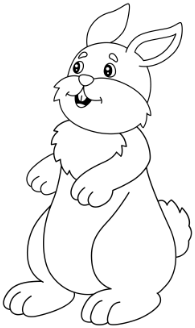
\includegraphics[height=3.2cm]{p16_tho.png}};}
        % 3 - 1: cà rốt
        \begin{scope}[shift={(8.9,0)}]
        \draw[PQkhung] (0,0) rectangle (8.3,5.1);
        \node[font=\sffamily\bfseries\fontsize{26}{26}\selectfont] at (3.3,4.45) {3 $-$ 1 $=$};
        \draw[line width=1.6pt] (5.1,4.1) -- (6.6,4.1);
        \foreach \x in {1.9,4.15,6.4}{\begin{scope}[shift={(\x,1.75)},scale=1.25]\PQcarotve{}\end{scope}}
        \end{scope}
        % 4 - 1: chú lùn
        \begin{scope}[shift={(0,-5.6)}]
        \draw[PQkhung] (0,0) rectangle (8.3,5.1);
        \node[font=\sffamily\bfseries\fontsize{26}{26}\selectfont] at (3.3,4.45) {4 $-$ 1 $=$};
        \draw[line width=1.6pt] (5.1,4.1) -- (6.6,4.1);
        \foreach \x in {1.3,3.2,5.1,7.0}{\node[inner sep=0pt] at (\x,1.85) {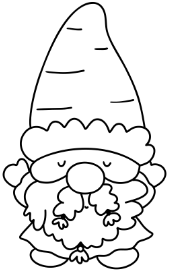
\includegraphics[height=2.95cm]{p16_chulun.png}};}
        \end{scope}
        % 5 - 3: đầu thỏ
        \begin{scope}[shift={(8.9,-5.6)}]
        \draw[PQkhung] (0,0) rectangle (8.3,5.1);
        \node[font=\sffamily\bfseries\fontsize{26}{26}\selectfont] at (3.3,4.45) {5 $-$ 3 $=$};
        \draw[line width=1.6pt] (5.1,4.1) -- (6.6,4.1);
        \foreach \x/\y in {1.0/1.05,2.6/2.35,4.15/1.05,5.7/2.35,7.3/1.05}{\begin{scope}[shift={(\x,\y)},scale=1.12]\PQdauthove\end{scope}}
        \end{scope}
    \end{tikzpicture}\par}
\end{bt}
\newpage
\begin{bt}
    Bé hãy quan sát các bạn khủng long bị gạch rồi viết phép trừ phù hợp.
    \TTbatdauhinh
    {\centering
        \PQokhunglong{PKcam}{-1.6/0.75/1,0/0.75/0,1.6/0.75/0,-0.8/-0.75/1,0.8/-0.75/0}\hfill
        \PQokhunglong{PQngoc}{-1.3/0.65/1,1.3/0.65/1,0/-0.7/1}\hfill
        \PQokhunglong{PQtim}{-1.3/0.65/1,1.3/0.65/1,0/-0.7/0}\\[12pt]
        \PQokhunglong{PKxanhla}{-1.1/-0.05/1,1.1/-0.05/0}\hfill
        \PQokhunglong{PKxanhnuoc}{-1.6/0.75/1,0/0.75/1,1.6/0.75/0,-0.8/-0.75/1,0.8/-0.75/0}\hfill
        \PQokhunglong{PKhong!90!red}{-1.2/0.75/0,1.2/0.75/0,-1.2/-0.75/0,1.2/-0.75/1}\par}
\end{bt}
\TTcachbai

\begin{bt}
    Bé hãy tìm đường đi trong mê cung.
    \TTbatdauhinh
    {\centering
    \begin{tikzpicture}
        \node[font=\bfseries] at (-2.6,5.85) {a)};
        \node[anchor=west,font=\itshape] at (-2.2,5.85) {Giúp ông già Noel lấy túi quà.};
        \begin{scope}[shift={(0,0)}]\PQmecung{(0,7)--(9,7) (0,6)--(1,6) (3,6)--(4,6) (5,6)--(7,6) (2,5)--(3,5) (2,4)--(3,4) (4,4)--(6,4) (6,3)--(8,3) (1,2)--(4,2) (6,2)--(7,2) (3,1)--(6,1) (8,1)--(9,1) (0,0)--(9,0) (0,7)--(0,6) (0,5)--(0,0) (1,6)--(1,1) (2,7)--(2,5) (2,3)--(2,2) (2,1)--(2,0) (3,5)--(3,3) (3,2)--(3,1) (4,6)--(4,3) (5,6)--(5,5) (5,4)--(5,1) (6,5)--(6,4) (6,3)--(6,2) (7,6)--(7,3) (7,2)--(7,0) (8,7)--(8,4) (8,3)--(8,2) (9,7)--(9,2) (9,1)--(9,0)}\end{scope}
        \begin{scope}[shift={(-1.45,4.15)}]\PQnoel\end{scope}
        \draw[-stealth,PKxanhla!80!black,line width=1.6pt] (-0.55,4.18) -- (0.2,4.18);
        \begin{scope}[shift={(7.95,1.14)}]\PQtuiqua\end{scope}
        % mê cung b
        \begin{scope}[shift={(0,-7.0)}]
        \node[font=\bfseries] at (-2.6,5.85) {b)};
        \node[anchor=west,font=\itshape] at (-2.2,5.85) {Giúp bạn người tuyết tìm lại chiếc mũi cà rốt.};
        \PQmecung{(0,7)--(9,7) (1,6)--(3,6) (4,6)--(5,6) (7,6)--(8,6) (3,5)--(4,5) (2,4)--(3,4) (4,4)--(6,4) (1,3)--(2,3) (6,3)--(8,3) (0,2)--(2,2) (7,2)--(9,2) (0,1)--(1,1) (2,1)--(3,1) (7,1)--(8,1) (0,0)--(9,0) (0,7)--(0,2) (0,1)--(0,0) (1,6)--(1,4) (2,5)--(2,3) (2,2)--(2,1) (3,6)--(3,5) (3,4)--(3,1) (4,7)--(4,6) (4,5)--(4,0) (5,6)--(5,5) (5,3)--(5,0) (6,6)--(6,1) (7,7)--(7,4) (7,2)--(7,1) (8,5)--(8,3) (9,7)--(9,6) (9,5)--(9,0)}
        \begin{scope}[shift={(-1.45,1.3)}]\PQnguoituyet\end{scope}
        \draw[-stealth,PKxanhla!80!black,line width=1.6pt] (-0.55,1.14) -- (0.2,1.14);
        \begin{scope}[shift={(8.1,4.18)}]\PQcarotmau\end{scope}
        \end{scope}
    \end{tikzpicture}\par}
\end{bt}

%---------- Bài bổ sung (Toán) ----------
\newpage
\begin{bt}
    Bé hãy quan sát tranh rồi viết phép trừ thích hợp.
    \TTbatdauhinh
    {\centering
    \begin{tikzpicture}[font=\sffamily\Large,scale=1.15]
        % a) cây thông có 5 quả châu, 2 quả rơi xuống
        \node[font=\bfseries] at (-0.9,3.3) {a)};
        \fill[gray!20] (1.6,-0.05) ellipse (2.2 and 0.15);
        \begin{scope}[shift={(1.2,0)},scale=0.95]\PQcaythong[0]
            \foreach \x/\y/\m in {-0.6/0.65/red,0.55/1.25/PKxanhnuoc,-0.2/2.0/PKvang}{\shade[ball color=\m] (\x,\y) circle (0.15);}
        \end{scope}
        \shade[ball color=red] (2.85,0.12) circle (0.15);
        \shade[ball color=PKvang] (3.4,0.12) circle (0.15);
        \draw[gray,thick,dashed,->] (2.05,1.35) to[bend left=25] (2.75,0.4);
        \draw[gray,thick,dashed,->] (2.0,0.9) to[bend left=25] (3.3,0.4);
        \foreach \x in {0,1.6,3.2}{\node[draw,thick,rounded corners=3pt,minimum size=0.95cm] at (\x,-1.1) {};}
        \node at (0.8,-1.1) {$-$}; \node at (2.4,-1.1) {$=$};
        % b) 4 chú chim trên cành, 1 chú bay đi
        \begin{scope}[shift={(8.6,0)}]
            \node[font=\bfseries] at (-0.9,3.3) {b)};
            \draw[PKnau,line width=4pt,line cap=round] (-0.6,1.0) .. controls (0.8,1.15) and (2.0,0.9) .. (3.4,1.05);
            \draw[PKnau,line width=2.5pt,line cap=round] (2.6,1.0) .. controls (2.9,0.6) .. (3.2,0.45);
            \foreach \x/\y in {1.0/0.35,2.2/0.0}{\fill[green!55!black,rotate around={-30:(\x,\y+0.95)}] (\x,\y+0.95) ellipse (0.22 and 0.09);}
            \foreach \x/\m in {-0.25/PKcam,0.65/PKxanhnuoc,1.55/PKvang,2.45/PKhong}{\begin{scope}[shift={(\x,1.42)},scale=1.05]\PQchim{\m}\end{scope}}
            \begin{scope}[shift={(3.55,2.75)},scale=1.05,rotate=15]\PQchim{PKxanhla}
                \fill[PKxanhla!60!black] (-0.05,0.05) -- (-0.25,0.42) -- (0.12,0.12) -- cycle;\end{scope}
            \draw[gray,thick,dashed,->] (2.6,2.0) to[bend left=25] (3.05,2.6);
            \foreach \x in {0,1.6,3.2}{\node[draw,thick,rounded corners=3pt,minimum size=0.95cm] at (\x,-1.1) {};}
            \node at (0.8,-1.1) {$-$}; \node at (2.4,-1.1) {$=$};
        \end{scope}
    \end{tikzpicture}\par}
\end{bt}
\TTcachbai

\begin{bt}
    Bé hãy tính rồi tô màu hộp quà theo kết quả: \textbf{0} -- \textcolor{PKxanhdam}{\textbf{xanh dương}}, \textbf{1} -- \textcolor{PKdo}{\textbf{đỏ}}, \textbf{2} -- \textcolor{green!50!black}{\textbf{xanh lá}}, \textbf{3} -- \textcolor{orange!90!black}{\textbf{vàng}}.
    \TTbatdauhinh
    {\centering
    \begin{tikzpicture}
        \foreach \so/\m [count=\k] in {0/PKxanhdam,1/PKdo,2/PKxanhla,3/PKvang}{
            \begin{scope}[shift={(3.4*\k-1.0,3.0)}]
                \shade[ball color=\m] (0,0) circle (0.3);
                \node[font=\sffamily\bfseries\Large,anchor=west] at (0.45,0) {$=$ \so};
            \end{scope}}
        \foreach \pt [count=\k] in {5 $-$ 4,4 $-$ 2,3 $-$ 0,2 $-$ 2,5 $-$ 3,4 $-$ 3,5 $-$ 2,3 $-$ 3}{
            \pgfmathtruncatemacro{\cot}{mod(\k-1,4)}\pgfmathtruncatemacro{\hang}{div(\k-1,4)}
            \begin{scope}[shift={(4.2*\cot+1.2,-3.0*\hang+0.4)},scale=1.25]\PQhopqua{\pt}\end{scope}}
    \end{tikzpicture}\par}
\end{bt}
\TTcachbai

\begin{bt}
    Đoàn tàu đếm lùi: bé hãy điền số còn thiếu vào các toa tàu.
    \TTbatdauhinh
    {\centering
        \PQtau{5}{4}{}{2}{}{0}\\[22pt]
        \PQtau{5}{}{3}{}{1}{}\par}
\end{bt}

%%%%%%%%%%%%%%%%%%%%%%%%%%%%%%%%%%%%%%%%%%%%%%%%%%%%%%%%%%
%                  PHIẾU TIẾNG VIỆT
%%%%%%%%%%%%%%%%%%%%%%%%%%%%%%%%%%%%%%%%%%%%%%%%%%%%%%%%%%
\newpage
\TTdatlaibai
{\centering
        {\color{mauchinh!120}\bfseries\Large PHIẾU BÀI TẬP TIẾNG VIỆT PRE1 -- TUẦN 16}\\[3pt]
        {\color{mauchinh!120}\bfseries\Large CHỦ ĐỀ 16: LÀM QUEN ÂM C, X}\par}
\vspace{6pt}
\TTthongtin

\begin{bt}
    Bé hãy đọc và khoanh vào âm \textbf{c} của các từ phía dưới.
    \TTbatdauhinh
    {\centering\PQchumau{C}{c}{0.8}\par}
    \TTbatdauhinh
    {\centering
        \PKbontranh{c}{p16_co.png}{con cò}{p16_coi.png}{cái cối}{p16_cam.png}{quả cam}{p16_cua.png}{con cua}\hfill
        \begin{minipage}[b]{0.42\linewidth}\centering\PKghep{c}{o}{co}\\[8pt]\PKghep{c}{ó}{có}\end{minipage}\par}
\end{bt}
\TTcachbai

\begin{bt}
    Bé hãy đọc và khoanh vào âm \textbf{x} của các từ phía dưới.
    \TTbatdauhinh
    {\centering\PQchumau{X}{x}{1.5}\par}
    \TTbatdauhinh
    {\centering
        \PKbontranh{x}{p16_xedap.png}{xe đạp}{p16_xucxich.png}{xúc xích}{p16_mamxoi.png}{mâm xôi}{p16_xoai.png}{quả xoài}\hfill
        \begin{minipage}[b]{0.42\linewidth}\centering\PKghep{x}{e}{xe}\\[8pt]\PKghep{x}{é}{xé}\end{minipage}\par}
\end{bt}
\newpage
\begin{bt}
    Bé hãy tô màu \textcolor{PKdo}{\textbf{đỏ}} vào củ cà rốt có chữ \textbf{c} và tô màu \textcolor{orange!90!black}{\textbf{cam}} vào củ cà rốt có chữ \textbf{x}.
    \TTbatdauhinh
    {\centering
    \begin{tikzpicture}
        \fill[gray!18] (8.0,-1.05) ellipse (3.2 and 0.24);
        \begin{scope}[shift={(8.0,-1.0)},scale=2.05]\PQcaythong
            \foreach \x/\y/\a/\b in {-1.0/0.12/PKdo/PKvang,0.98/0.1/PKxanhnuoc/PKdo,-0.55/-0.02/PKvang/PKxanhla}{
                \fill[\a,draw=\a!60!black,thin] (\x-0.22,\y-0.17) rectangle (\x+0.22,\y+0.17);
                \fill[\b] (\x-0.04,\y-0.17) rectangle (\x+0.04,\y+0.17);
                \fill[\b] (\x-0.22,\y-0.025) rectangle (\x+0.22,\y+0.025);
                \fill[\b] (\x,\y+0.17) .. controls (\x-0.15,\y+0.33) and (\x-0.22,\y+0.26) .. (\x,\y+0.17) .. controls (\x+0.15,\y+0.33) and (\x+0.22,\y+0.26) .. (\x,\y+0.17);}
        \end{scope}
        \foreach \x/\y/\c/\g in {0.7/5.4/c/-20,3.3/4.6/x/-12,0.5/2.6/x/-28,3.1/1.9/c/-15,0.8/-0.2/c/-30,3.4/-0.7/x/-18,
                                 12.7/4.6/c/12,15.3/5.4/x/20,12.9/1.9/x/15,15.5/2.6/c/28,12.6/-0.7/c/18,15.2/-0.2/x/30}{
            \begin{scope}[shift={(\x,\y)},rotate=\g,scale=0.98]\PQcarotve{\c}\end{scope}}
    \end{tikzpicture}\par}
\end{bt}
\TTcachbai

\begin{bt}
    Bé hãy nối mỗi hình với chữ \textbf{c} hoặc chữ \textbf{x} có trong tên gọi.
    \TTbatdauhinh
    {\centering
    \begin{tikzpicture}
        \foreach \hinh/\ten [count=\k] in {p16_cumeo.png/cú mèo,p16_mixao.png/mì xào,p16_xedap2.png/xe đạp}{
            \begin{scope}[shift={(0,-3.9*\k+3.9)}]\PQthe{\hinh}{\ten}\fill (1.75,-0.25) circle (2.6pt);\end{scope}}
        \foreach \hinh/\ten [count=\k] in {p16_cucai.png/củ cải,p16_cao.png/con cáo,p16_q_xoai.png/quả xoài}{
            \begin{scope}[shift={(15.0,-3.9*\k+3.9)}]\PQthe{\hinh}{\ten}\fill (-1.75,-0.25) circle (2.6pt);\end{scope}}
        \begin{scope}[shift={(7.5,-0.6)}]\PQvongsong{c}\fill (-1.2,0) circle (2.6pt); \fill (1.2,0) circle (2.6pt);\end{scope}
        \begin{scope}[shift={(7.5,-7.2)}]\PQvongsong{x}\fill (-1.2,0) circle (2.6pt); \fill (1.2,0) circle (2.6pt);\end{scope}
    \end{tikzpicture}\par}
\end{bt}
\newpage
\begin{bt}
    Bé hãy điền \textbf{c} hoặc \textbf{x} vào chỗ chấm rồi đọc to các từ.
    \TTbatdauhinh
    {\centering
        \PQodien{\PQanh{p16_ca.png}}{con \PQtrong{}á}\hfill
        \PQodien{\PQanh{p16_xoi.png}}{đĩa \PQtrong{}ôi}\hfill
        \PQodien{\PQanh{p16_cachua.png}}{quả \PQtrong{}à chua}\\*[10pt]
        \PQodien{\PQanh{p16_xe.png}}{\PQtrong{}e ô tô}\hfill
        \PQodien{\begin{scope}[scale=1.05]\PQco\end{scope}}{lá \PQtrong{}ờ}\hfill
        \PQodien{\begin{scope}[scale=1.15]\PQxo\end{scope}}{cái \PQtrong{}ô}\par}
\end{bt}
\TTcachbai

\begin{bt}
    Bé hãy đọc tên các loại quả, nối tên quả có \textbf{dấu huyền} với dấu huyền ở giữa.
    \TTbatdauhinh
    {\centering
    \begin{tikzpicture}
        \fill[PKvangnhat!60,draw=black!70,thick] (0,0) circle (1.15);
        \draw[line width=7pt,line cap=round] (-0.3,0.45) -- (0.3,-0.35);
        \foreach \hinh/\ten/\x/\y/\dx/\dy [count=\k] in {p16_q_chuoi.png/chuối/-2.4/4.0/-1.35/1.65,p16_q_hong.png/hồng/2.4/4.0/1.35/1.65,
                                              p16_q_xoai.png/xoài/6.0/1.75/3.55/0.75,p16_q_buoi.png/bưởi/6.0/-1.85/3.55/-0.75,
                                              p16_q_dau.png/dâu/2.4/-4.1/1.35/-1.75,p16_q_dua.png/dừa/-2.4/-4.1/-1.35/-1.75,
                                              p16_q_oi.png/ổi/-6.0/-1.85/-3.55/-0.75,p16_q_tao.png/táo/-6.0/1.75/-3.55/0.75}{
            \node[inner sep=0pt] (q\k) at (\x,\y) {\includegraphics[height=1.6cm,width=2.0cm,keepaspectratio]{\hinh}};
            \node[draw,thick,rounded corners=4pt,fill=PKvangnhat,inner sep=3pt,minimum width=1.7cm,anchor=north,font=\large] at ([yshift=-2pt]q\k.south) {\ten};
            \fill (\dx,\dy) circle (2.6pt);}
    \end{tikzpicture}\par}
\end{bt}

\newpage % trang tập viết chữ c
\begin{bt}
    Bé hãy viết chữ \textbf{c}.
    \PQoli{c}{6}{5}
\end{bt}

\newpage % trang tập viết chữ x
\begin{bt}
    Bé hãy viết chữ \textbf{x}.
    \PQoli{x}{6}{5}
\end{bt}

%---------- Bài bổ sung (Tiếng Việt) ----------
\newpage
\begin{bt}
    Bé hãy nhìn tranh và khoanh vào tiếng viết đúng.
    \TTbatdauhinh
    {\centering
    \begin{tikzpicture}[font=\Large]
        \foreach \hinh/\a/\b [count=\k] in {p16_ca.png/cá/xá,p16_xe.png/ce/xe,p16_cua.png/cua/xua,p16_xoi.png/côi/xôi,
                                           p16_co.png/xò/cò,p16_cam.png/cam/xam,p16_cao.png/cáo/xáo,p16_q_xoai.png/coài/xoài}{
            \pgfmathtruncatemacro{\cot}{mod(\k-1,4)}\pgfmathtruncatemacro{\hang}{div(\k-1,4)}
            \begin{scope}[shift={(4.2*\cot,-3.6*\hang)}]
                \draw[thick,rounded corners=8pt,fill=PKvangnhat!35] (-1.85,-1.55) rectangle (1.85,1.4);
                \node[inner sep=0pt] at (0,0.4) {\includegraphics[height=1.6cm,width=2.9cm,keepaspectratio]{\hinh}};
                \node at (-0.85,-1.05) {\a};
                \node at (0.85,-1.05) {\b};
            \end{scope}}
    \end{tikzpicture}\par}
\end{bt}
\TTcachbai

\begin{bt}
    Bé hãy tô màu các ô có chữ \textbf{c} để giúp bạn cua tìm đường về hang.
    \TTbatdauhinh
    {\centering
    \begin{tikzpicture}
        \fill[PQcat!35,rounded corners=12pt] (-2.2,-5.85) rectangle (12.6,0.8);
        \foreach \r [count=\i] in {{c,c,x,o,x,a,e},{x,c,c,c,o,x,c},{a,x,e,c,x,c,c},{o,e,x,c,c,c,x},{x,a,o,x,e,a,o}}{
            \foreach \chu [count=\j] in \r {\PQoChu{1.35*\j-1.0,-1.3*\i+1.3}{\chu}}}
        \node[inner sep=0pt] at (-1.25,0.0) {
\includegraphics[height=1.15cm]{p16_cua.png}};
        \draw[-stealth,PKxanhla!80!black,line width=1.4pt] (-0.55,0.0) -- (-0.25,0.0);
        \draw[-stealth,PKxanhla!80!black,line width=1.4pt] (9.2,-1.3) -- (9.55,-1.3);
        \begin{scope}[shift={(10.75,-1.05)},scale=1.05]\PQhangcua\end{scope}
    \end{tikzpicture}\par}
\end{bt}

\begin{center}
       \faGg\faGg\quad Hết \quad\faGg\faGg
\end{center}
\end{document}
